\documentclass[border=6pt]{standalone}
\usepackage{amsmath}
\usepackage{tikz}
\usetikzlibrary{arrows.meta}
\begin{document}
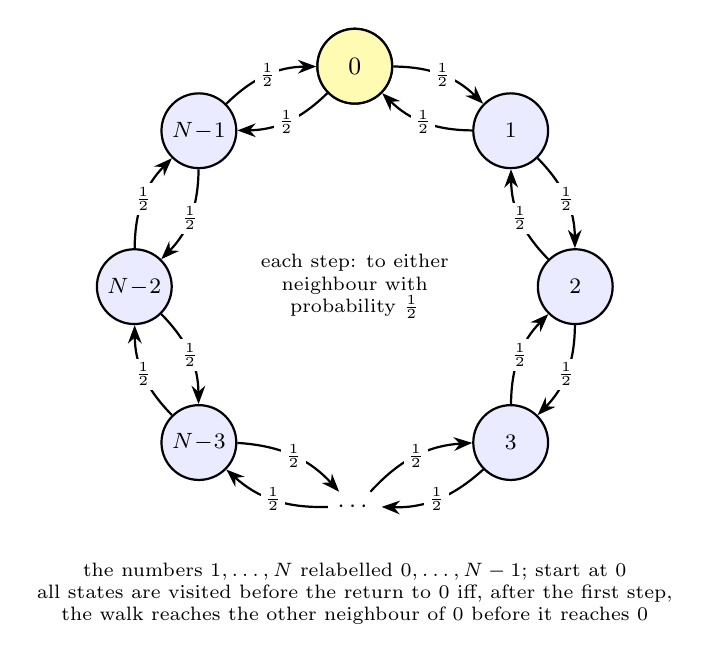
\begin{tikzpicture}[>=Stealth,font=\small,
 s/.style={draw,thick,circle,minimum size=1.1cm,inner sep=0pt,fill=blue!8},
 e/.style={->,thick},
 lab/.style={font=\small,fill=white,inner sep=1.5pt},
 every loop/.style={->,thick,looseness=6}]
\def\R{2.8}
\foreach \i/\t/\a in {0/0/90,1/1/45,2/2/0,3/3/-45,4/\cdots/-90,5/N\!-\!3/-135,6/N\!-\!2/180,7/N\!-\!1/135} {
  \ifnum\i=4 \node (v\i) at (\a:\R) {$\t$};
  \else \node[s,minimum size=0.95cm,font=\footnotesize] (v\i) at (\a:\R) {$\t$}; \fi
}
\node[s,minimum size=0.95cm,fill=yellow!30] at (90:\R) {$0$};
\foreach \i/\j in {0/1,1/2,2/3,3/4,4/5,5/6,6/7,7/0} {
  \draw[e] (v\i) to[bend left=22] node[lab,font=\scriptsize]{$\tfrac12$} (v\j);
  \draw[e] (v\j) to[bend left=22] node[lab,font=\scriptsize]{$\tfrac12$} (v\i);
}
\node[font=\scriptsize,align=center] at (0,0) {each step: to either\\neighbour with\\probability $\tfrac12$};
\node[font=\scriptsize,align=center] at (0,-3.9) {the numbers $1,\dots,N$ relabelled $0,\dots,N-1$; start at 0\\all states are visited before the return to 0 iff, after the first step,\\the walk reaches the other neighbour of 0 before it reaches 0};
\end{tikzpicture}
\end{document}
